eCAD also provides the option to select the entities. User may select the entities either through the mouse clicks or through the Select Menu.
\subsection{Using Mouse}
eCAD allows the user to select one or multiple entities.
\begin{enumerate}
\item \textbf{Selecting single entity:} User may select single entity by simply clicking on that entity.
\begin{figure}[h!]
\centering
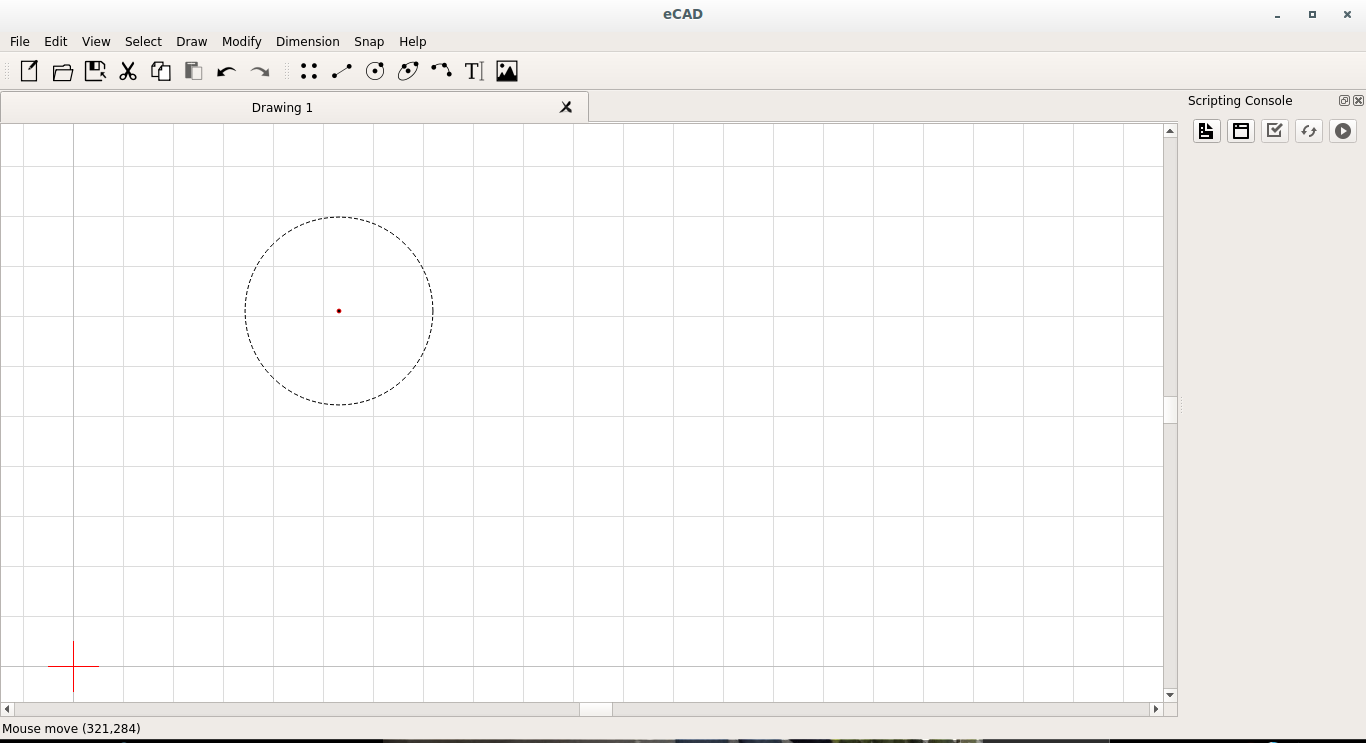
\includegraphics[width=0.5\textwidth]{images/mouseSelect.png}
\end{figure}
\item \textbf{Selecting multiple entities:} Dragging the mouse over the entities will allow one to select them.
\begin{figure}[h!]
\centering
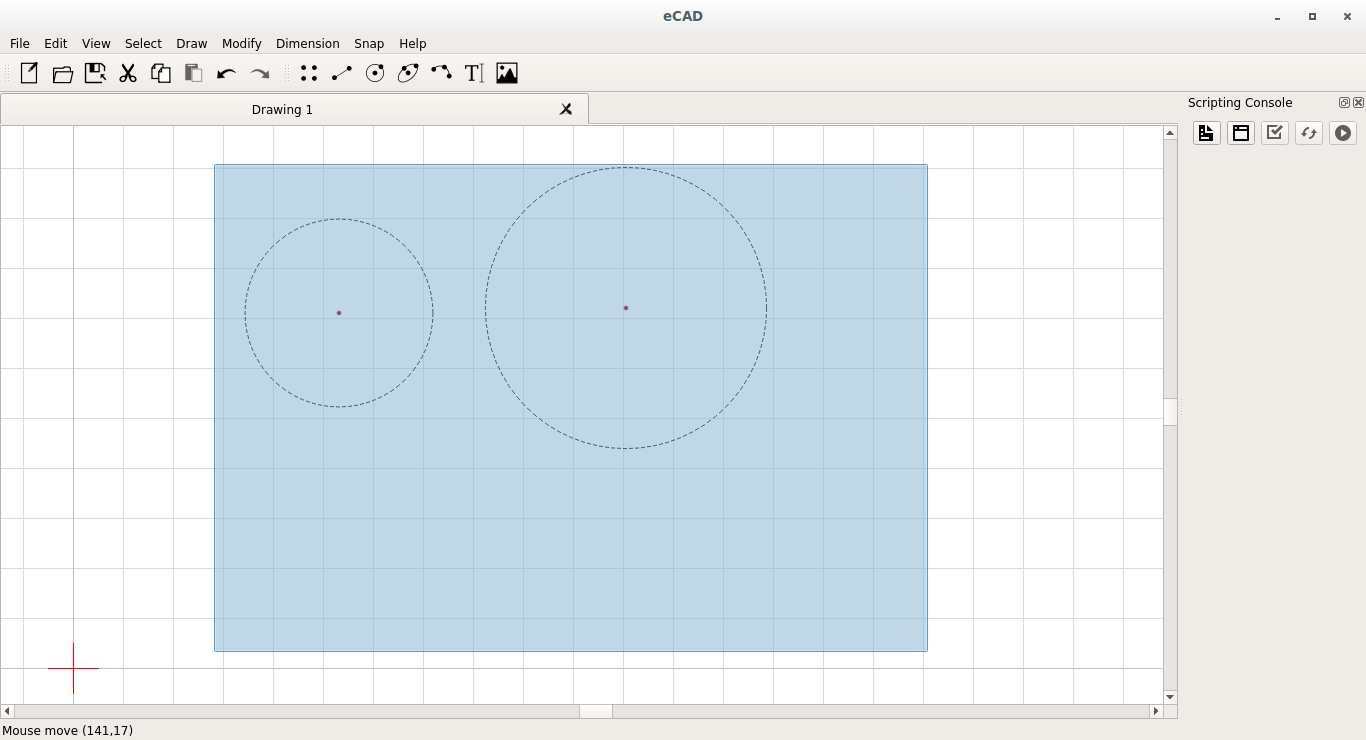
\includegraphics[width=0.5\textwidth]{images/multiple.png}
\end{figure}
\end{enumerate}
\subsection{Select Menu}
Select Menu provides various options to select the entities. Select menu options are explained below:
\begin{enumerate}
\item \textbf{Select All:} This option allows to select all the entities that are currently present on the workspace.
\item \textbf{DeSelect All:} This option allows to deselect all the entities that were currently selected.
\item \textbf{Select Entity:} This option is valid for the single entity that provides user to select the entity, if there is only one entity currently visible.
\item \textbf{Select Window:} Clicking this option would give a user a message to drag the mousein the drawing area to make selection using window and you may drag the mousein to make selection.
\begin{figure}[h!]
\centering
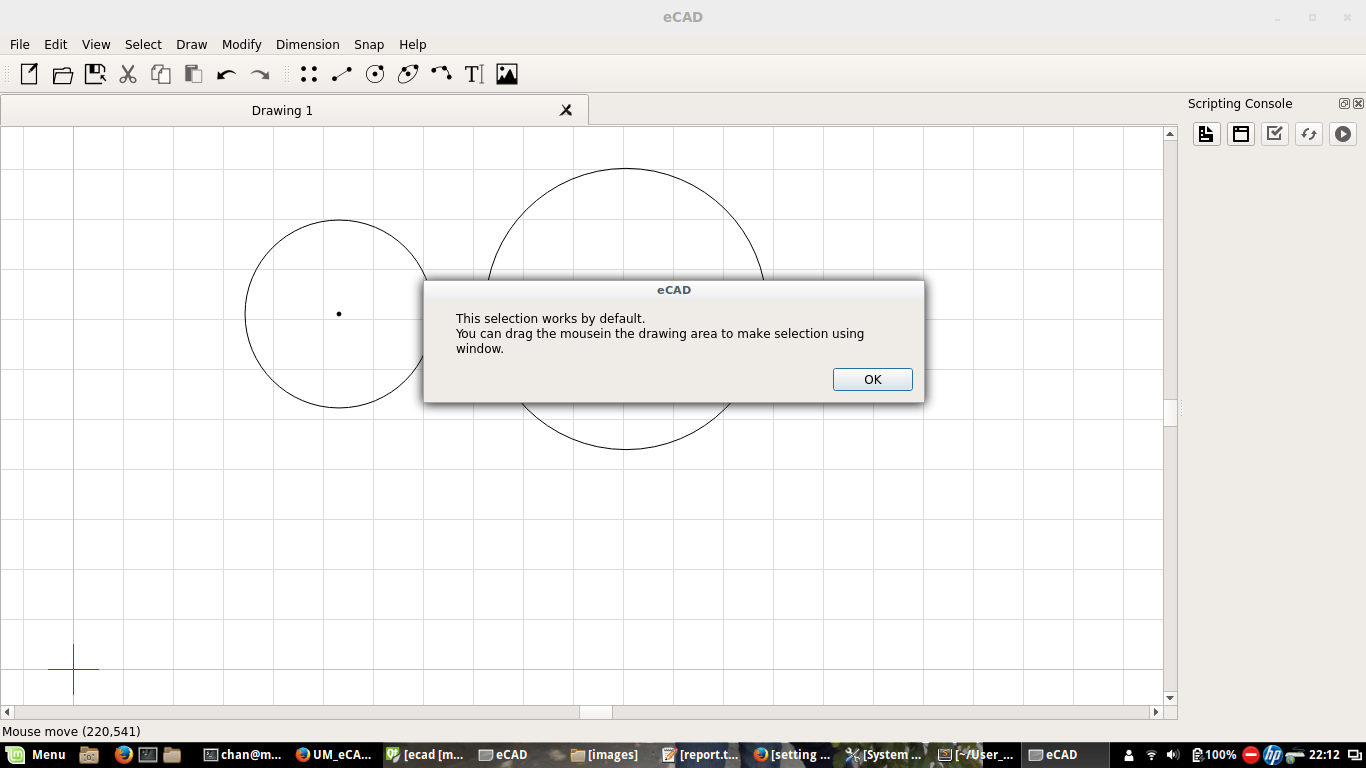
\includegraphics[width=0.9\textwidth]{images/messsage.png}
\end{figure}
\item \textbf{DeSelect Window:} This would allow the user to deselect the entities, selected using Select Window.
\item \textbf{Invert Selection:} Invering selection will make selected entities deselected and vice versa.
\end{enumerate}